\documentclass[a4paper, 12pt]{report}
%\usepackage{portuguese}{babel}
\usepackage{subfiles}
\usepackage{forloop}
\usepackage{arydshln}
\usepackage{fancyhdr}
\usepackage{graphicx}
\usepackage{booktabs}
\graphicspath{ {./assets/} }

\title {Desenvolvimento de Sistemas de Software}

% CAPA COM ID + GRUPO
\author{\textbf{Grupo 31} \\
        \begin{tabular} { c c }
                
\includegraphics[scale=0.4]{author/marco.jpg} & 
\includegraphics[scale=0.4]{author/marco.jpg} \\
                62608 - Marco Sousa                           & 93198 - Mariana Marques                       \\
                \hline \\
                
\includegraphics[scale=0.4]{author/marco.jpg} & 
\includegraphics[scale=0.4]{author/marco.jpg} \\
                93271 - José Malheiro                         & 94269 - Miguel Fernandes
        \end{tabular}
}

\begin{document}
\maketitle

\begin{abstract}
        Lorem ipsum dolor sit amet, consectetur adipiscing elit. Proin rhoncus, eros et pellentesque vestibulum, nulla quam fermentum mauris, eget viverra metus massa ut libero. Proin vel pellentesque lectus, vitae viverra sapien. Nullam interdum condimentum malesuada. Cras in odio et leo pharetra dapibus sit amet ut turpis. Cras consequat quam nec diam sollicitudin dignissim. Suspendisse ante mi, pulvinar dapibus interdum sed, vulputate a quam. Etiam a fermentum purus. Curabitur posuere nisl sed tempor varius. Donec vestibulum leo purus, id placerat lacus efficitur ac. Lorem ipsum dolor sit amet, consectetur adipiscing elit. Cras dui nisl, rutrum at venenatis ac, rutrum vestibulum justo. Phasellus sodales pharetra sapien, et mattis nulla maximus sed. Ut placerat ultricies molestie. Integer feugiat euismod faucibus.


        descrição
        e
        objetivos
\end{abstract}

% breve descrição proposto + objetivos desta fase
% objetivos: modelo de domínio
% abordagem seguida para os atingir - reunir em grupo e fazer
% resultados obtidos - modelos desenvolvidos
\section{Modelação de Domínio}
% adicionar o modelo de Domínio
% adicionar descrição do modelo
\subsection{Entidades}

\begin{itemize}
        \item[Cliente]{} % NIF
        \item[Colaborador] {} %% prazo máximo de reparação ; Preço
        \item[Equipamento] {} %% Código de registo
        \item[Orçamento] {}
        \item[Reparação] {} % Reparação normal - Passo da Reparação, tempo, peças/ material utilizadas - calculo do preço através do material (ter uma tabela)
              % Reparação expresso - Preço fixo; serviços disponíveis?
        \item[Forma de Contacto] {}
\end{itemize}
% Cliente

% Orçamento

% Equipamento



%%% 
% Colaborador
%% Funcionário do Balcão
%% Técnico
%% Gestor
% Formas de Contacto
%% SMS
%% Email

% descrição das entidades
\subsection{Diagrama de Modelo de Domínio} % diagrama ?? anexo ??

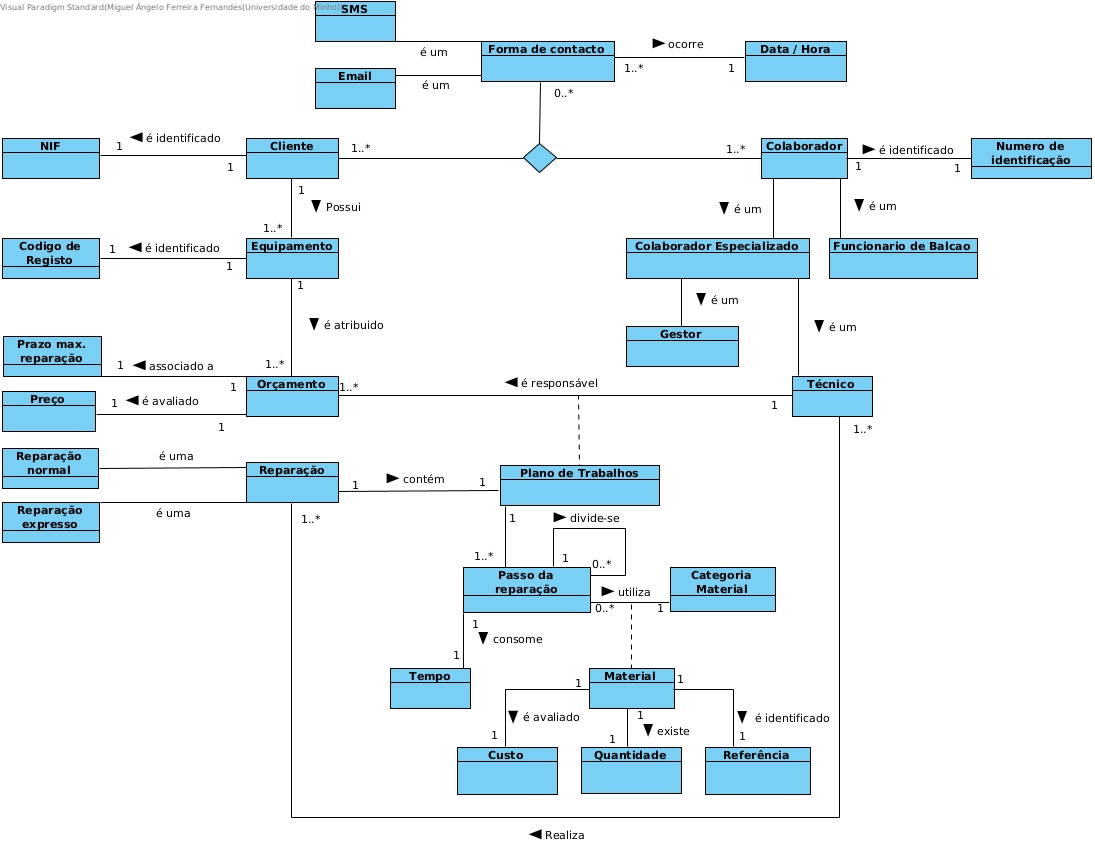
\includegraphics[scale=0.41]{Modelo.jpg}

\section{Modelação dos Requisitos Funcionais}
% O que o sistema deve fazer
Cenários foram identificados pela equipa docente.
% adicionar o diagrama de use case
A partir dos cenários foram identificados os seguintes \textit{use cases}:
\begin{itemize}
        \item Pedir orçamento - \ref{pedir_orcamento}
        \item Fazer orçamento - \ref{fazer_orcamento}
        \item Confirmar orçamento - \ref{confirmar_orcamento}
        \item Arquivar orçamento - \ref{arquivar_orcamento}
        \item Realizar reparação - \ref{realizar_rep}
        \item Entregar equipamento - \ref{entregar_equipamento}
        \item Pedir reparação expresso - \ref{pedir_rep_xpress}
        \item Registar equipamento - \ref{registar_equipamento}
        \item Registar cliente - \ref{registar_cliente}
        \item Listar resumida do técnico - \ref{listagem_tecnico_resumida}
        \item Listar detalhada do técnico - \ref{listagem_tecnico_detalhada}
        \item Listar funcionário do balcão - \ref{listagem_func_balcao}
\end{itemize}
\subsection{Modelo de Use Cases} % anexo ??

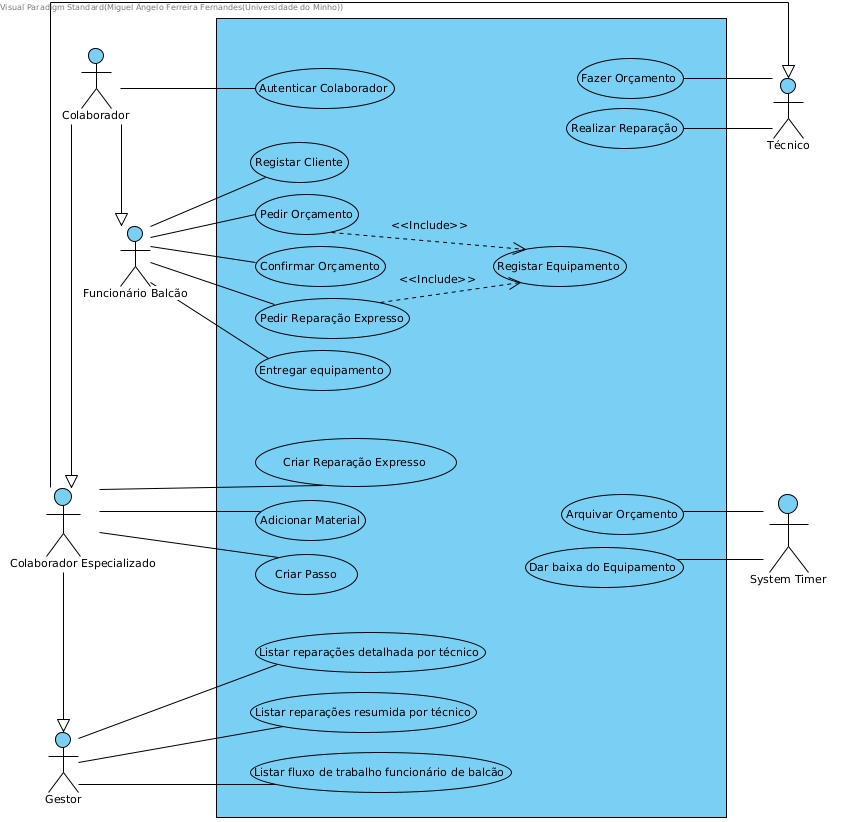
\includegraphics[scale=0.45]{dss-usecase.jpg}

\subsection{Especificação Use Cases}

\subsubsection{} \label{pedir_orcamento}
\subfile{use_cases/usecase_pedir-orcamento.tex}

\subsubsection{} \label{fazer_orcamento}
\subfile{use_cases/usecase_fazer-orcamento.tex}

\subsubsection{} \label{confirmar_orcamento}
\subfile{use_cases/usecase_confirmar-orcamento.tex}

\subsubsection{} \label{arquivar_orcamento}
\subfile{use_cases/usecase_arquivar-orcamento.tex}

\subsubsection{} \label{realizar_rep}
\subfile{use_cases/usecase_realizar-reparacao.tex}

\subsubsection{} \label{entregar_equipamento}
\subfile{use_cases/usecase_entregar-equipamento.tex}

\subsubsection{} \label{pedir_rep_xpress}
\subfile{use_cases/usecase_pedir-reparacao-expresso.tex}

\subsubsection{} \label{registar_equipamento}
\subfile{use_cases/usecase_registar-equipamento.tex}

\subsubsection{} \label{registar_cliente}
\subfile{use_cases/usecase_registar-cliente.tex}

\subsubsection{} \label{listagem_tecnico_resumida}
\subfile{use_cases/usecase_listar-tecnico-resumida.tex}

\subsubsection{} \label{listagem_tecnico_detalhada}
\subfile{use_cases/usecase_listar-tecnico-detalhada.tex}

\subsubsection{} \label{listagem_func_balcao}
\subfile{use_cases/usecase_listar-func-balcao.tex}

\section{Considerações Finais}
% análise crítica dos resultados

\end{document}